%NEURAL PRESY ;)

%----------------------------------------------------------------------------------------
%   PACKAGES AND THEMES
%----------------------------------------------------------------------------------------

\documentclass{beamer}

\mode<presentation> {

% The Beamer class comes with a number of default slide themes
% which change the colors and layouts of slides. Below this is a list
% of all the themes, uncomment each in turn to see what they look like.

%\usetheme{default}
%\usetheme{AnnArbor}
%\usetheme{Antibes}
%\usetheme{Bergen}
\usetheme{Berkeley}
%\usetheme{Berlin}
%\usetheme{Boadilla}
%\usetheme{CambridgeUS}
%\usetheme{Copenhagen}
%\usetheme{Darmstadt}
%\usetheme{Dresden}
%\usetheme{Frankfurt}
%\usetheme{Goettingen}
%\usetheme{Hannover}
%\usetheme{Ilmenau}
%\usetheme{JuanLesPins}
%\usetheme{Luebeck}
%\usetheme{Madrid}
%\usetheme{Malmoe}
%\usetheme{Marburg}
%\usetheme{Montpellier}
%\usetheme{PaloAlto}
%\usetheme{Pittsburgh}
%\usetheme{Rochester}
%\usetheme{Singapore}
%\usetheme{Szeged}
%\usetheme{Warsaw}

% As well as themes, the Beamer class has a number of color themes
% for any slide theme. Uncomment each of these in turn to see how it
% changes the colors of your current slide theme.

%\usecolortheme{albatross}
%\usecolortheme{beaver}
%\usecolortheme{beetle}
%\usecolortheme{crane}
%\usecolortheme{dolphin}
%\usecolortheme{dove}
%\usecolortheme{fly}
%\usecolortheme{lily}
%\usecolortheme{orchid}
%\usecolortheme{rose}
%\usecolortheme{seagull}
%\usecolortheme{seahorse}
%\usecolortheme{whale}
%\usecolortheme{wolverine}

%\setbeamertemplate{footline} % To remove the footer line in all slides uncomment this line
%\setbeamertemplate{footline}[page number] % To replace the footer line in all slides with a simple slide count uncomment this line

\setbeamertemplate{navigation symbols}{} % To remove the navigation symbols from the bottom of all slides uncomment this line
}

\usepackage{graphicx} % Allows including images
\graphicspath{ {images/} }
\usepackage{booktabs} % Allows the use of \toprule, \midrule and \bottomrule in tables
\usepackage{caption}
\usepackage{subcaption}
\usepackage{algorithm,algorithmic}
\usepackage{pgfplots}

\def\layersep{2cm}
\def\nodesep{0.25cm}
\usepackage{tikz, calc}
\newcommand*{\Scale}[2][4]{\scalebox{#1}{$#2$}}%
\newcommand*{\Resize}[2]{\resizebox{#1}{!}{$#2$}}%
\newcommand\sep{1.9cm}
\newcommand\height{0.9cm}
\usetikzlibrary{decorations.pathmorphing, backgrounds}
\tikzset{snake it/.style={decorate, decoration=snake}}
%

%----------------------------------------------------------------------------------------
%   TITLE PAGE
%----------------------------------------------------------------------------------------

\title[OpenBrain]{OpenBrain}

%\author{William Guss}
\date{April 22, 2016} % Date, can be changed to a custom date
\makeatletter
\newcommand{\verbatimfont}[1]{\renewcommand{\verbatim@font}{\ttfamily#1}}
\makeatother
\begin{document}

\begin{frame}
\titlepage
\end{frame}

\begin{frame}

\begin{center}
\Huge 
\end{center}

\frametitle{Overview}
\tableofcontents
\end{frame}

%----------------------------------------------------------------------------------------
%   PRESENTATION SLIDES
%----------------------------------------------------------------------------------------

%------------------------------------------------
\section{Organization} % Sections can be created in order to organize your presentation into discrete blocks, all sections and subsections are automatically printed in the table of contents as an overview of the talk
%-----------------------------------------------

    \begin{frame}
        \frametitle{Current Work Session Organization}
        We currently have three sets of separate meetings throughout the week.
        \begin{enumerate}
        \item Algorithms Meeting - Tuesday Evenings - talk strictly about the different pieces of the OpenBrain model.
        \item Reading group - Friday Afternoons - First hour spent on presenting the paper to the group; Second hour spent on discussing what elements could be incorporated into the OpenBrain model.
        \item Software Meeting - Monday afternoons. Discuss implementation details and write code.
        \begin{enumerate}
        \item These have unfortunately been infrequent 
        \end{enumerate}
        \end{enumerate}
       
    \end{frame}
\section{Theory}
    \begin{frame}
        \frametitle{Theory: Important Concerns}
        	\begin{enumerate}
	        	\item Intelligence - definition and measurement
                \begin{itemize}
					\item UIM incompatable:
                    \begin{equation}
                  \Upsilon(\pi) = \sum_{\mu \in E}2^{-K(\mu)}  \mathbb{E}\left(\sum_{i=1}^\infty r_i \right) 
                  \end{equation}
                  requires meaningful "timesteps", $\pi_O$ runs asynchronously!
                \end{itemize}
                \item Mathematical framework for asynchronicity.
                \begin{itemize}
                \item How do we talk about representation theory for agent on different timeline.
                \end{itemize}
                \item Conwayian learning rules for emergent intelligence
                \begin{enumerate}
                	\item Especially stressing the need to keep emergent rules simple.
                \end{enumerate}
            \end{enumerate}
    \end{frame}



 


    \begin{frame}
    \frametitle{Theory: A Rigorous Mathematical Framework}
    \emph{How do we account for asynchronousity?} Ignore it! \\[0.25cm]
\begin{centering}

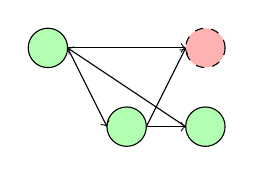
\begin{tikzpicture}
  \draw[style=dashed, fill=red!30] (2,.5) circle (0.25);
  \draw[fill=green!30] (1,-0.5) circle (0.25);
  \draw[fill=green!30] (2,-0.5) circle (0.25);
  \draw[fill=green!30] (0,0.5) circle(0.25);
  \path[draw, ->] (0.25,0.5) -- (1.75,.5) ;
  \path[draw, ->] (0.25, 0.5) -- (0.75,-0.5) ;
  \path[draw, ->] (1.25,-0.5) -- (1.75,.5);
   \path[draw, ->]  (1.75,-.5) -- (0.25, 0.5)  ;
  \path[draw, ->] (1.25,-0.5) -- (1.75,-.5);
\end{tikzpicture} 

\end{centering}
 \textbf{Definition.}
  A \textbf{neuron} $n \in N$ is defined by
  \begin{itemize}
    \item a voltage $V_n(t)$
    \item a decay time $\tau_n$
    \item a refactory period $\rho_n$
    \item a voltaic threshold $\theta_n$
  \end{itemize}
  \textbf{Definition.}
  A \textbf{connection} $c \in C$ is a tuple $(n_i, n_j, w_{ij}) \in N \times N \times \mathbb{R}$
  where $n_i$ is  the \textbf{anterior neuron}, $n_j$ is the \textbf{posterior neuron}, and $w_ij$
  is the standard synaptic weight.

    \end{frame}


    \begin{frame}
    \frametitle{Theory: A Rigorous Mathematical Framework} 

    \begin{columns}
      \begin{column}{0.7\textwidth}
\textbf{Definiton. }
  A neuron $n$ is said to \textbf{fire} if it is not in its refractory period and $V_n(t_{k}) = V_n[k] > \theta_n$. Then for all $m \in P_n$,
  \begin{equation*}
    V_m[k+1] {\ +_=\ } w_{nm} \sigma(V_n[k]); \label{eq:fire}
  \end{equation*}
  that is, voltage is propagated to the posterior neurons.  \\[0.5cm]

  Immediately after neuron $n$ fires, it enters  a \textbf{refractory period} until time $t_{k} + \rho_n$, or iteration $k + \frac{\rho_n}{\Delta t}$. 

      \end{column}
      \begin{column}{0.3\textwidth}
      \begin{figure}
          \begin{centering}
            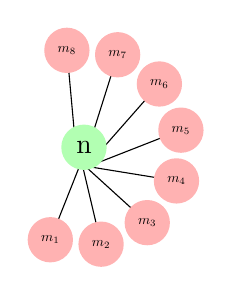
\begin{tikzpicture}
              \foreach \a in {1,2,...,8}{
              \path[draw, ->] (\a*360/6: 0.25cm)  -- (\a*360/12 + 220: 1.5cm-0.25cm) node[circle, fill=red!30, scale=1] {$\Scale[0.5]{m_{\a}}$};
              
              }
            \node[circle, style=dashed, fill=green!30] {n};
          \end{tikzpicture} 

          \end{centering}
          \caption{A neuron $n$ firing  into its posterior neurons, $P_n = \{m_1, \dots, m_8\}$}
      \end{figure}
      
      \end{column}
    \end{columns}
    \end{frame}

       \begin{frame}
    \frametitle{Theory: Continuous Time Universal Intelligence}
    \begin{itemize}
      \item Theoretical problems evaluating our agent.
      \item UIM defines an environment, $\mu$, as a probability measure on sequences of actions and perceptions. Typically
      \begin{equation}
        o_1r_1a_1o_2r_2a_2\dots o_nr_na_n          
       \end{equation}   
       where $r_i$ are rewards!
       \item What does it mean to have a reward at time step $k$ when $\Delta t \to 0$? \textbf{$\pmb{r_i} \pmb{\to} \pmb{0}$ :(}
       \item Actions become sparse as $\Delta t \to 0.$
       \begin{equation}
         a_1\emptyset\dots\dots\dots\emptyset a_{100000} \emptyset \dots\dots \emptyset a_{2500605}\dots
        \end{equation} 
    \end{itemize}
    \end{frame}


    \begin{frame}

      \frametitle{Theory: Continuous Time Universal Intelligence} 

      \begin{figure}
        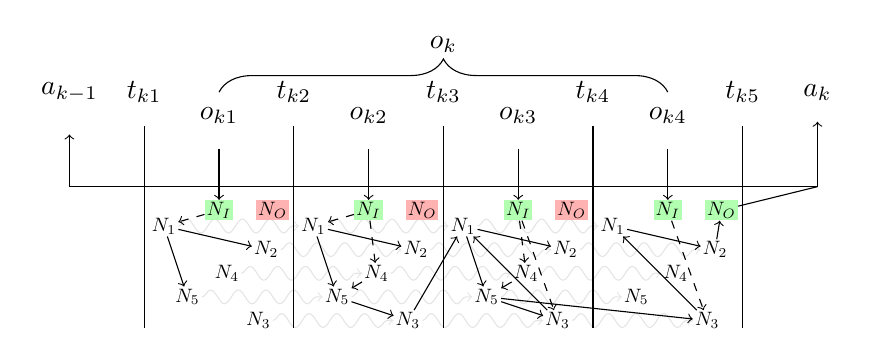
\begin{tikzpicture}

        % Top nodes
        \node[circle, fill=white] (akm1) at (0,\height + 0.3cm ) {$\pmb{a_{k-1}}$} ;
         \foreach \a in {1,2,3,4}{
          \node[circle, fill=white] (ok\a) at (\a*\sep,\height) {$o_{k\a}$} ;

          \node[circle, fill=white] (ok\a) at (\a*\sep,\height) {$o_{k\a}$} ;
        }


        \node[circle, fill=white] (ak) at (5*\sep,\height+0.3cm ) {$\pmb{a_{k}}$} ;


        %Generate neurons
        \foreach \a in {1,2,3,4}{
          \node[ scale=0.7, fill=green!30, inner sep=1pt] (NI\a) at (\a*\sep,-0.3) {$N_I$} ;
          \path[draw, ->] (ok\a) -- (NI\a);

          \node[ scale=0.7, inner sep=1pt,] (N1\a) at (\a*\sep -0.7cm,-0.5) {$N_1$} ;
          \node[ scale=0.7, inner sep=1pt,] (N2\a) at (\a*\sep +0.6cm,-0.8) {$N_2$} ;
          \node[ scale=0.7, inner sep=1pt,] (N3\a) at (\a*\sep +0.5cm,-1.7) {$N_3$} ;
          \node[ scale=0.7, inner sep=1pt,] (N4\a) at (\a*\sep +0.1cm,-1.1) {$N_4$} ;
          \node[ scale=0.7, inner sep=1pt,] (N5\a) at (\a*\sep -0.4cm,-1.4) {$N_5$} ;
          \node[ scale=0.7, fill=red!30, inner sep=1pt ] (NO\a) at (\a*\sep +0.68cm,-0.3) {$N_O$} ;



        }
        \node[ scale=0.7, fill=green!30, inner sep=1pt ] (NO4) at (4*\sep +0.68cm,-0.3) {$N_O$} ;


        %WEIGHT DEQAY
        \foreach \a in {1,2,3}{
            \foreach \b in {1,2,3,4,5}{
            \begin{scope}[on background layer]
            \pgfmathsetmacro\q{int(\a + 1)}
              \path[draw, color=gray!20, ->, snake it] (N\b\a) -- (N\b\q) ;
              \end{scope}
              
            }
        }

        %NEURO FIRINGS
        \path[draw, ->, dashed] (NI1) -- (N11);
        \path[draw, ->] (N11) -- (N21);
        \path[draw, ->] (N11) -- (N51);

        \path[draw, ->, dashed] (NI2) -- (N12);
        \path[draw, ->, dashed] (NI2) -- (N42);
        \path[draw, ->] (N12) -- (N22);
        \path[draw, ->] (N12) -- (N52);
        \path[draw, ->] (N42) -- (N52);
        \path[draw, ->] (N52) -- (N32);
        \path[draw, ->] (N32) -- (N13);

        \path[draw, ->, dashed] (NI3) -- (N33);
        \path[draw, ->, dashed] (NI3) -- (N43);
        \path[draw, ->] (N43) -- (N53);
        \path[draw, ->] (N53) -- (N33);
        \path[draw, ->] (N33) -- (N13);
        \path[draw, ->] (N13) -- (N53);
        \path[draw, ->] (N13) -- (N23);
        \path[draw, ->] (N53) -- (N34);

        \path[draw, ->, dashed] (NI4) -- (N34);
        \path[draw, ->] (N34) -- (N14);
        \path[draw, ->] (N14) -- (N24);
        \path[draw, ->] (N24) -- (NO4);
        \path[draw, -] (NO4) -- (\sep*5,0);




        %TIME!
                \foreach \a in {1,2,...,5} {
          \node[circle, fill=white] (tka\a) at (\a*\sep -\sep/2,\height+0.3cm) {$t_{k\a}$} ;
          \path[draw, -] (tka\a) -- +(0,-3); 
        }
        
        
        %a bridge.
        \path[draw, <->] (akm1) -- +(0,-\height -0.3cm) -- (5*\sep,0)  -- (ak);

      \draw [decorate,decoration={brace,amplitude=12pt},xshift=-0pt]
      (\sep,\height+0.3cm) -- (4*\sep,\height+0.3cm) node [black,midway,yshift=.6cm] 
      { $\pmb{o_k}$};



      \end{tikzpicture} 
        \caption{The diagram of sub-observation neural interaction for $\pi_O$.}
      \end{figure}

      \textbf{Solution: Subobservations}
      \begin{itemize}
        \item  Actions determine what it means to be an observation.   
        \item A visualization of asyncronous neural activity.
        \item More details in our paper at github. 
      \end{itemize}
    \end{frame}


    \begin{frame}
    \frametitle{Theory: Other progress!}
    	\begin{enumerate}
            \item Hutter's AIXI
            \item Biological parallels:
           	\begin{enumerate}
            	\item Synaptogenesis
                \item Asynchronicity - important
                \item Refractory periods
            \end{enumerate}
           \item Sparse Distributed Representation
           \item LSTM Models: Rewards associated with actions taken in the world.
           \item In the process of writing paper to be presented at NIPS (2017) conference.
        \end{enumerate}
    \end{frame}
    \begin{frame}
   	\frametitle{Theory: Goals}
    	\begin{enumerate}
       		\item Develop a strong representation theory for the algorithm.
          \begin{enumerate}
              \item What class of functions can OpenBrain approximate?         
          \end{enumerate}
            \item Figuring out how to measure learning quantitatively
            \item Expanding framework to include specialized neurons to more closely mimic biology
            	\begin{enumerate}
                	\item Wide variety of applications to all sorts of problems if specificity can be 							cracked.
					\item Cracking neuron specificity and learning $\rightarrow$ solution to general AI 							problem as $t \to \infty$.
                \end{enumerate}
        \end{enumerate}
    \end{frame}
    \section{Software}

    \begin{frame}
    	\frametitle{Software: Overview}
    	The pieces of the OpenBrain software project
	    \begin{enumerate}
          \item Brain
          \item Environment
          \item Visualization
        \end{enumerate}
    \end{frame}
    
    \begin{frame}
    	\frametitle{Progress}
        \begin{enumerate}
          
          \item Design Doc Mostly Complete
          \item Prototyping Framework
          \begin{enumerate}
              \item Make sure that we can input learning rules 	
              \item Return empirical measurements to gauge usefulness of learning rules.
          \end{enumerate}
          \item Migrate to IDE
          \begin{enumerate}
              \item More efficient build process
              \item Code completion is nice
          \end{enumerate}
		\end{enumerate}
    \end{frame}
    \begin{frame}
    \Huge{\centerline{DEMO!!}}
    \end{frame}
    \begin{frame}
    \frametitle{Software: Obstacles}
    \begin{enumerate}
    \item Determining how to scale across many different computers
    \begin{enumerate}
	    \item How to scale program
        \item Designing for scale
    \end{enumerate}
    \item Saving state
    \item Maintaining inheritence patterns for neuron structures.
    \item Erlang is hard to learn
    \end{enumerate}
    \end{frame}
   

\begin{frame}
\frametitle{References}
\footnotesize{
    \begin{thebibliography}{99} % Beamer does not support BibTeX so references must be inserted manually as below
        \bibitem[Taigman, 2012]{p1} Yaniv Taigman et. al. (2014)
        \newblock DeepFace: Closing the Gap to Human-Level Performance in Face Verification
        \newblock \emph{Facebook AI Research}
        \bibitem[Nielsen , 2014]{p1} Michael Nielsen (2014)
        \newblock Neural Networks and Deep Learning
        \newblock \emph{http://neuralnetworksanddeeplearning.com/}
        
    \end{thebibliography}
}
\end{frame}

%------------------------------------------------

\begin{frame}
\Huge{\centerline{The End}}
\end{frame}

%----------------------------------------------------------------------------------------

\end{document}
